\documentclass[]{beamer}
%\documentclass[handout]{beamer}
%\documentclass[handout,draft]{beamer}
%\documentclass[]{article}


% Preambulo
% Paquetes para usar bien el idioma español
\usepackage[spanish,es-tabla]{babel}
\selectlanguage{spanish}
\usepackage[utf8]{inputenc}

% Paquetes para usar mejores imagenes
\usepackage{graphicx}

% Paquetes para links y tabla de contenidos en el PDF
\usepackage{hyperref}
\hypersetup{colorlinks=true,allcolors=blue}
%\usepackage{hypcap}

% Paquetes para mejores tablas
\usepackage{booktabs}

% Mejor matematica
\usepackage{amsmath}

% Fuentes de las imagenes
\usepackage[absolute,overlay]{textpos}

% Paquete captions
\usepackage[justification=centering,labelformat=empty,labelsep=none]{caption}

% Opciones para ticks
\usepackage{tikz}
\usetikzlibrary{shapes,arrows,positioning}

\tikzstyle{decision} = [diamond, draw, fill=blue!20, text width=4em, text badly centered, node distance=2cm, inner sep=0pt,on grid]
\tikzstyle{block} = [rectangle, draw, fill=blue!20, text width=8em, text centered, rounded corners, minimum height=2em,on grid]
\tikzstyle{line} = [draw, -latex]

% Citas bibliograficas
\usepackage[backend=biber]{biblatex}
\renewcommand{\footnotesize}{\tiny}
\addbibresource{biblio.bib}

% Mejoro las captions
\setbeamertemplate{caption}{\raggedright\insertcaption\par}

\setbeamertemplate{caption}{%
\begin{beamercolorbox}[wd=0.85\paperwidth, sep=.2ex]{block body}\insertcaption%
\end{beamercolorbox}%
}


% Sacar barra de navegacion
\setbeamertemplate{navigation symbols}{}%remove navigation symbols

% Transparencias en items
\setbeamercovered{transparent}

% Estilo de diapositivas
% \usetheme{Boadilla}
\usecolortheme{whale}
\usecolortheme{orchid}

%\usepackage{beamerarticle}

% Titulo
\title{Herramientas de Teledetección Cuantitativa\\{\small Rebotando por la atmósfera}}
\author{Francisco Nemiña}

\institute{Unidad de Educación y Formación Masiva \\
Comisión Nacional de Actividades Espaciales}

\logo{
\includegraphics[height=0.7cm]{imagenes/sopi.png}}

\AtBeginSection[]
{
\begin{frame}
\frametitle{Esquema de presentación}
\tableofcontents[currentsection]
\end{frame}
}


\begin{document}
\begin{frame}
    \maketitle
\end{frame}

\section{Escenas del capítulo anterior}
\begin{frame}{La vez pasada vimos}
  \begin{itemize}[<+->]
    \item Como partiendo de la energía se llega a la radiancia.
    \item Que la radiancia era una magnitud de interes pues es lo que media el sensor.
    \item Que la reflectancia se definia como $\rho = \pi L / E_0 \cos\theta$
    \item Que a partir de esto podiamos definir la $\rho_\lambda$ la firma espectral como una característica de cada cuerpo.
    \item Definimos 3 tipos de firmas espectrales \emph{patrón} y como se comportaba cada una.
  \end{itemize}
\end{frame}
%--- Next Frame ---%

\begin{frame}{Firmas espectrales}
  \begin{figure}
  \centering
  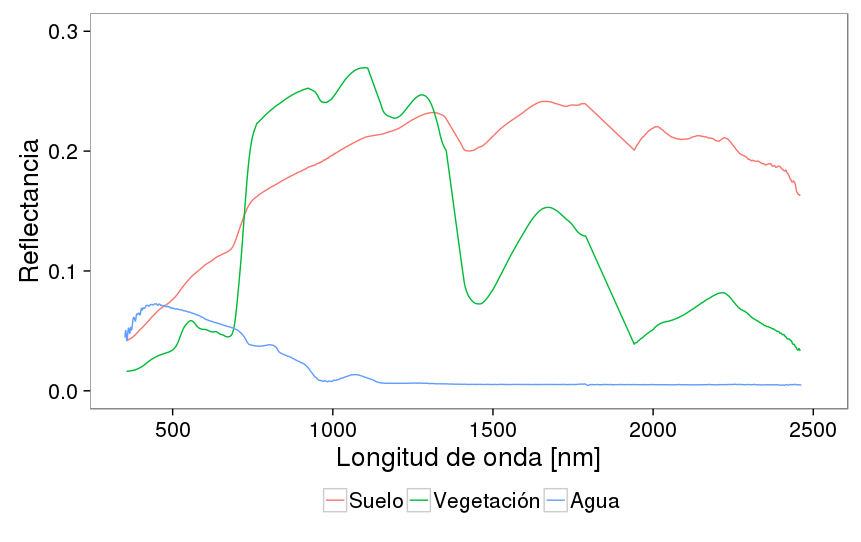
\includegraphics[width=0.8\textwidth]{imagenes/sig_tres.png}
  \caption{Firmas espectrales típicas de suelo, agua y vegetación.\footfullcite{clark2007usgs}}
  \end{figure}
\end{frame}
%--- Next Frame ---%

\section{Describiendo el problema}

\begin{frame}{Planteo del problema}
  \begin{block}{Problema}
    Queremos estudiar el problema de adquirir una imagen satelital teniendo en cuenta el efecto de la atmósfera.\pause
    Para esto estudiaremos la variación de la radiancia.
    $$L_\lambda$$
  \end{block}
\end{frame}
%--- Next Frame ---%

\begin{frame}{Interacciones}
  En la atmósfera pueden darse 3 tipos de interacción con la luz\pause
    \begin{itemize}[<+->]
      \item Absorción $\alpha$
      \item Transmisión $\tau$
      \item Dispersión $\rho$
    \end{itemize}\pause
    \begin{block}{Observación}
      \begin{equation}
        \alpha + \tau + \rho = 1
      \end{equation}
    \end{block}
\end{frame}
%--- Next Frame ---%

\begin{frame}{Visto en la atmósfera}
  \begin{figure}
  \centering
  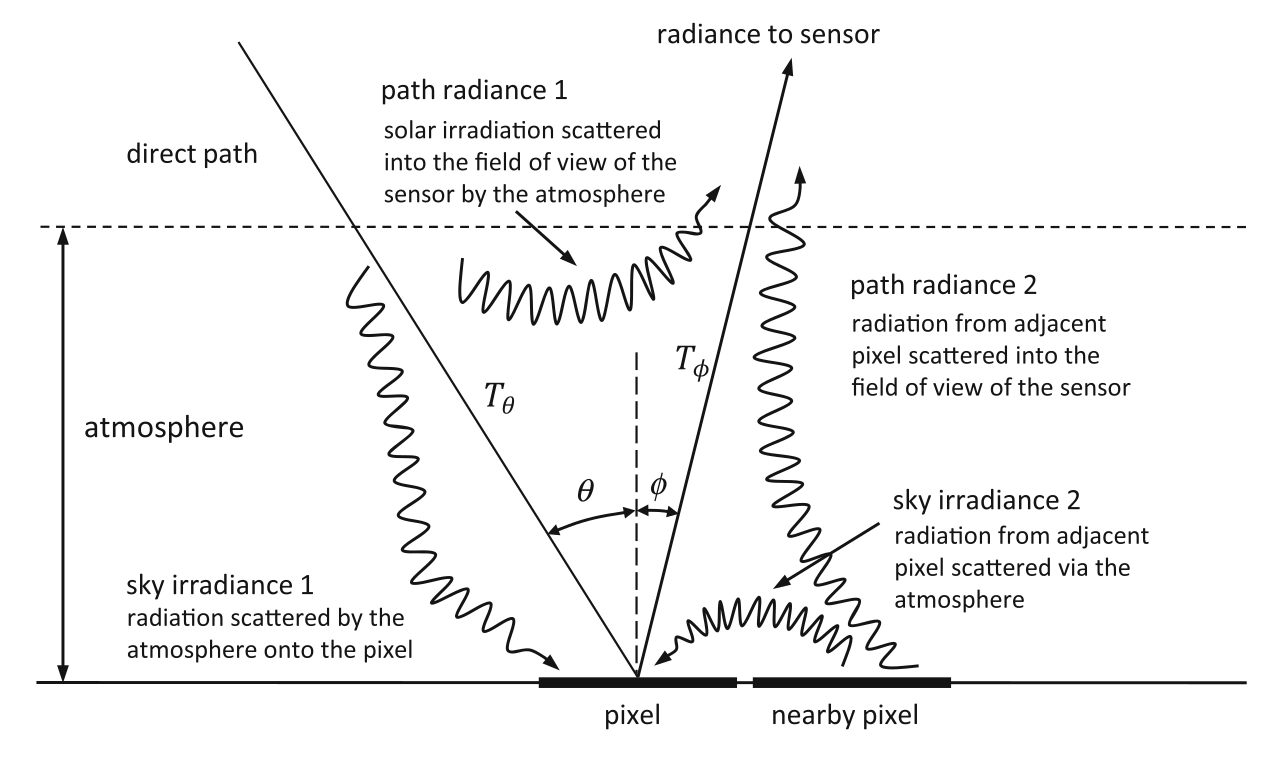
\includegraphics[width=0.8\textwidth]{imagenes/iatmo.png}
  \caption{Interacciones entre la atmósfera y la luz.\footfullcite{richards2013remote}}
  \end{figure}
\end{frame}
%--- Next Frame ---%

\begin{frame}{Planteo del problema}
  \begin{figure}
  \centering
  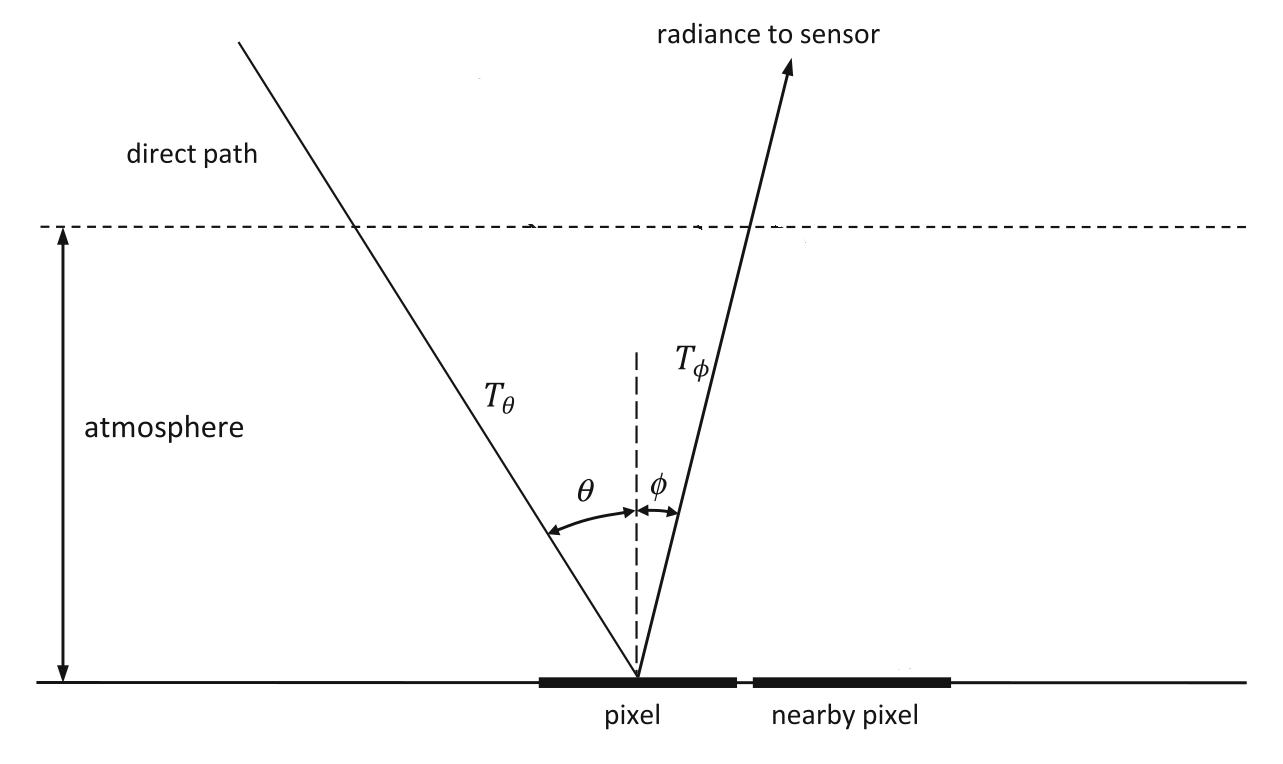
\includegraphics[width=0.8\textwidth]{imagenes/tatmo.png}
  \caption{Diagrama esquemático de la absorción en la atmósfera.\footfullcite{richards2013remote}}
  \end{figure}
\end{frame}
%--- Next Frame ---%

\begin{frame}{Planteo del problema}
  \begin{figure}
  \centering
  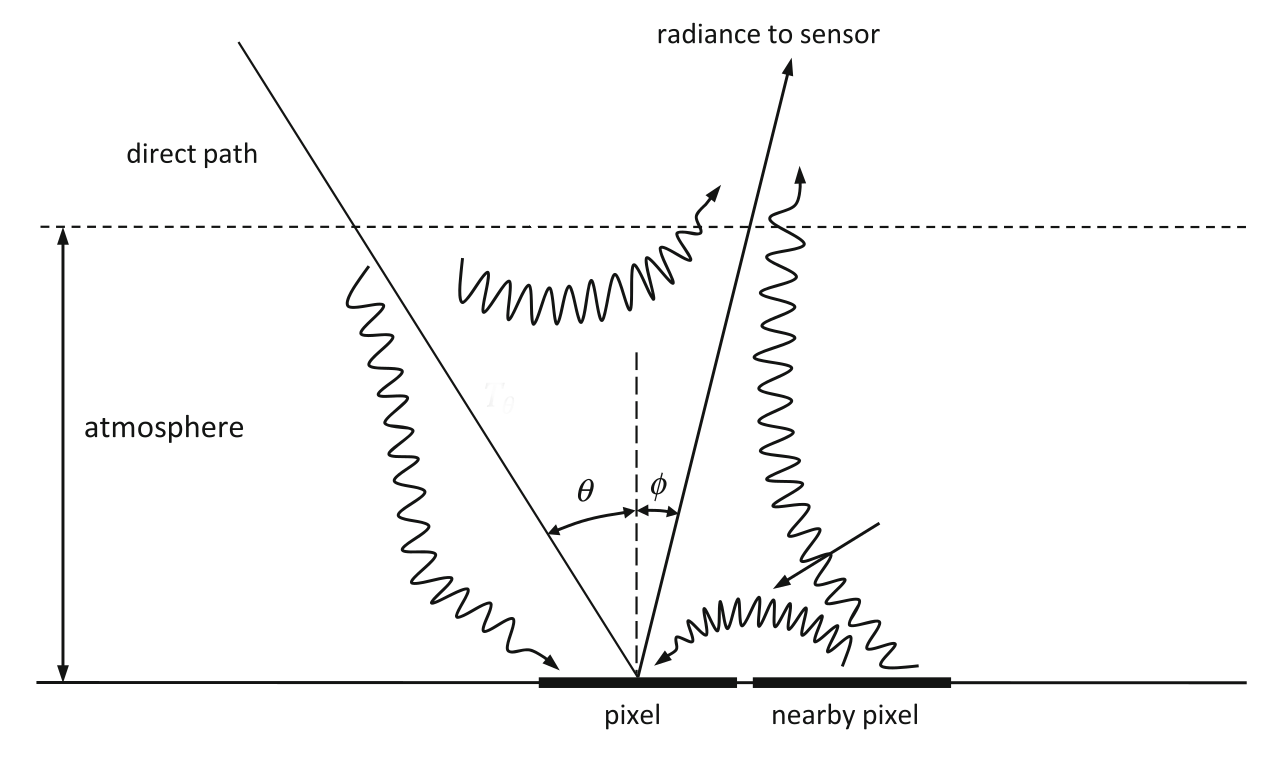
\includegraphics[width=0.8\textwidth]{imagenes/patmo.png}
  \caption{Diagrama esquemático de las dispersiones en la atmósfera.\footfullcite{richards2013remote}}
  \end{figure}
\end{frame}
%--- Next Frame ---%

\begin{frame}{Planteo del problema}
  \begin{block}{Formulación matemática}
    $$d L_\lambda = -k_\lambda \rho L_\lambda ds + j_\lambda \rho ds$$
    donde $-k_\lambda \rho L_\lambda ds$ representa absorciones y $j_\lambda \rho ds$ representa fuentes, \pause
    $$ \frac{dL_\lambda}{k_\lambda \rho ds} = -L_\lambda + J_\lambda$$
  \end{block}
  \pause
  \begin{block}{Nombres}
    \begin{itemize}
      \item $k_\lambda$ mass extintion cross section
      \item $j_\lambda$ source function coefficient
      \item $\rho$ densidad
    \end{itemize}
  \end{block}
\end{frame}
%--- Next Frame ---%

\begin{frame}{Planteo del problema}
  \begin{alertblock}{Aproximaciones}
    \begin{itemize}[<+->]
      \item Resolver esto en general no se puede.
      \item Hay que hacer distintas aproximaciones
    \end{itemize}
  \end{alertblock}
\end{frame}
%--- Next Frame ---%

\section{Aproximaciones}

\begin{frame}{Absorción constante y sin fuentes}
  \begin{exampleblock}{$k_\lambda = cte$, $j_\lambda = 0$}
    En este caso nos queda la ecuación
    \begin{equation}
        dL_\lambda = -k_\lambda \rho L_\lambda ds
    \end{equation}
    \pause cuya solución es
    \begin{equation}
        L_\lambda(s_1) = L_\lambda(0) \exp\left( -\int_0^{s_1} k_\lambda \rho ds \right)
    \end{equation}
  \end{exampleblock}
\end{frame}
%--- Next Frame ---%

\begin{frame}{Absorción constante y sin fuentes}
  \begin{exampleblock}{$k_\lambda = cte$, $j_\lambda = 0$}
    Un ejemplo de aplicación de esto es en batimetría.
    \begin{equation}
      s = m_1\times \frac{\log L_i}{\log L_j}+m_0
    \end{equation}
  \end{exampleblock}
\end{frame}

%--- Next Frame ---%
\begin{frame}{Absorción constante y sin fuentes}
  \begin{exampleblock}{$k_\lambda = cte$, $j_\lambda = 0$}
    \begin{figure}
    \centering
    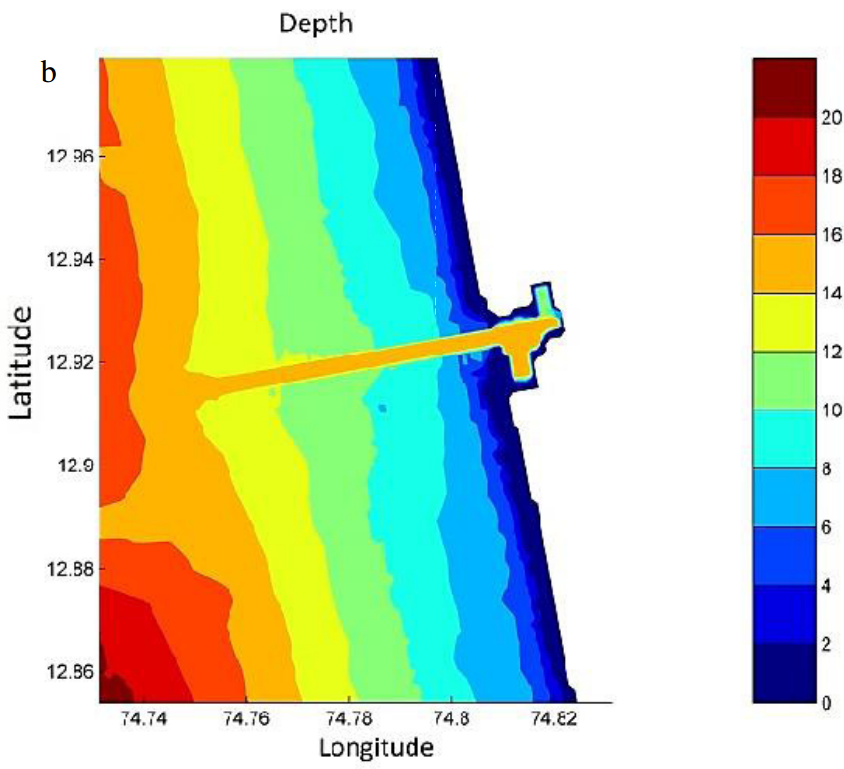
\includegraphics[width=0.5\textwidth]{imagenes/bati.png}
      \caption{Batimetría con Landsat 8.\footfullcite{jagalingam2015bathymetry}}
    \end{figure}
  \end{exampleblock}
\end{frame}
%--- Next Frame ---%

\begin{frame}{Atmósfera plana}
  \begin{exampleblock}{Atmósfera plana}
    Suponemos que toda la dependencia espacial es en la dirección z, entonces
    \begin{equation}
      \mu \frac{dL_\lambda}{k_\lambda \rho dz} = -L_\lambda + J_\lambda
    \end{equation} \pause
    definiendo a la profundidad óptica como
    \begin{equation}
        \tau_\lambda = \int_z^\infty k_\lambda \rho dz
    \end{equation}
  \end{exampleblock}
\end{frame}
%--- Next Frame ---%

\begin{frame}{Atmósfera plana}
  \begin{exampleblock}{Atmósfera plana}
    Nos queda entonces
    \begin{equation}
      \mu \frac{dL_\lambda}{d\tau} = L_\lambda - J_\lambda
    \end{equation}\pause
    Resolver esto ya depende de la atmósfera y no suele haber formas cerradas.
  \end{exampleblock}
  \pause
  \begin{alertblock}{Observación}
    Necesito además conocer 2 condiciones de contorno.
    \begin{itemize}[<+->]
      \item La radiancia solar
      \item La reflectancia en el terreno
    \end{itemize}
  \end{alertblock}
\end{frame}
%--- Next Frame ---%

\begin{frame}{Definiciones}
  \begin{block}{Definición}
    Llamamos \emph{transmitancia} $T$ a la fracción de radiancia que atraviesa la atmósfera dividida la radiancia incidente.
  \end{block}\pause
  \begin{block}{Defininción}
    Llamamos \emph{Irradiancia del cielo} a la cantidad de irradiancia $E_D$ que proviene del cielo e ilumina al píxel.
  \end{block}
  \pause
  \begin{block}{Defininción}
    Llamamos \emph{Radiancia de camino} a la cantidad de radiancia $L_P$ que proviene del cielo y viaja hacia el sensor.
  \end{block}
\end{frame}
%--- Next Frame ---%

\begin{frame}{Cálculo de la radiancia TOA}
  Con estas definiciones podemos calcular la radiancia recibida por el satélite como
  \begin{equation}
    L = T_\phi \frac{(E_0 T_\theta \cos \theta + E_D)\rho}{\pi} + L_p
  \end{equation}\pause
  Ahora tenémos que entender bien que representa cada cosa.
\end{frame}

\section{Dispersión}
\begin{frame}{Dispersión}
  La luz dispersada por la atmósfera provendrá de dos fuentes
  \begin{itemize}
    \item Moléculas
    \item Aerosoles
  \end{itemize}
\end{frame}
\begin{frame}{Dispersión}
  \begin{figure}
  \centering
  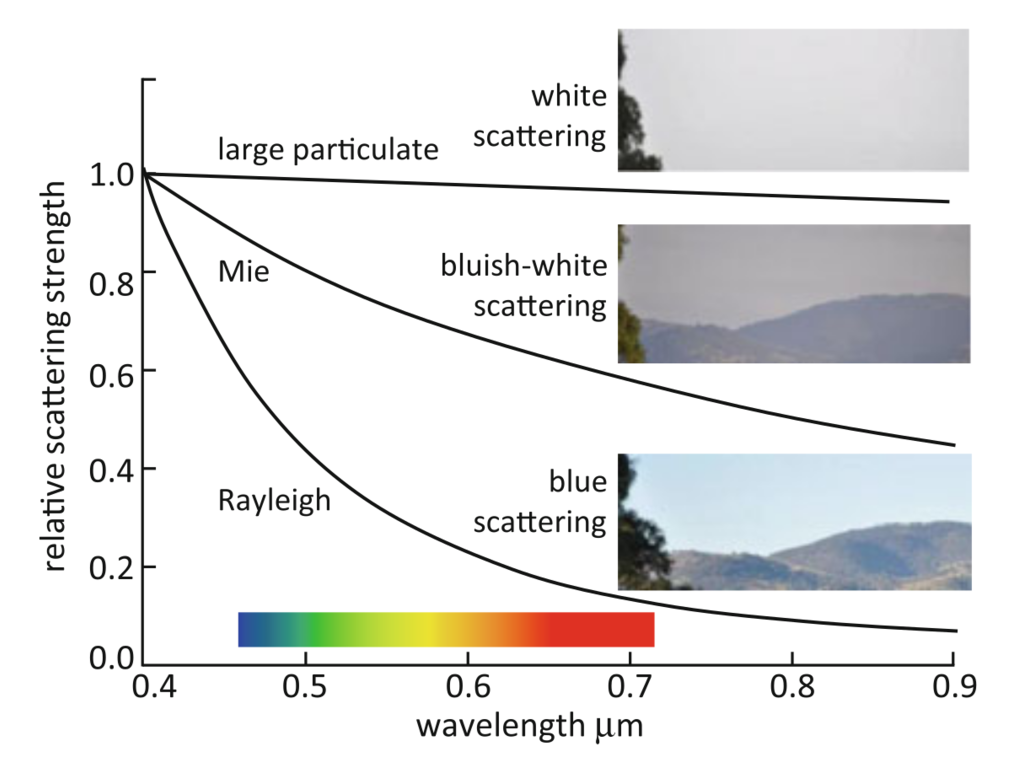
\includegraphics[width=0.8\textwidth]{imagenes/dispersion.png}
  \caption{Distintos tipos de dispersión en la atmósfera.\footfullcite{richards2013remote}}
  \end{figure}
\end{frame}
%--- Next Frame ---%
%--- Next Frame ---%
\subsection{Moléculas}
\begin{frame}{Moléculas}
  \begin{itemize}
    \item Está presente siempre.
    \item Es mas sencilla de modelar
  \end{itemize}
\end{frame}
%--- Next Frame ---%
\begin{frame}{Modelo de Rayleigh}
  Cuando las partículas tienen un tamaño mucho menor que la longitud de donde utilizada
  \begin{equation}
    L = L_0 \left( \frac{\lambda}{\lambda_0} \right)^{-4}
  \end{equation}
\end{frame}
%--- Next Frame ---%

\begin{frame}{Modelo de Rayleigh}
  \begin{itemize}[<+->]
    \item La existencia de esta dispersión, además, va a generar absorción en la atmósfera.
    \item La distribución angular no va a ser uniforme.
  \end{itemize}
\end{frame}
%--- Next Frame ---%

\begin{frame}{Sobre la firma espectral}
  \begin{figure}
  \centering
  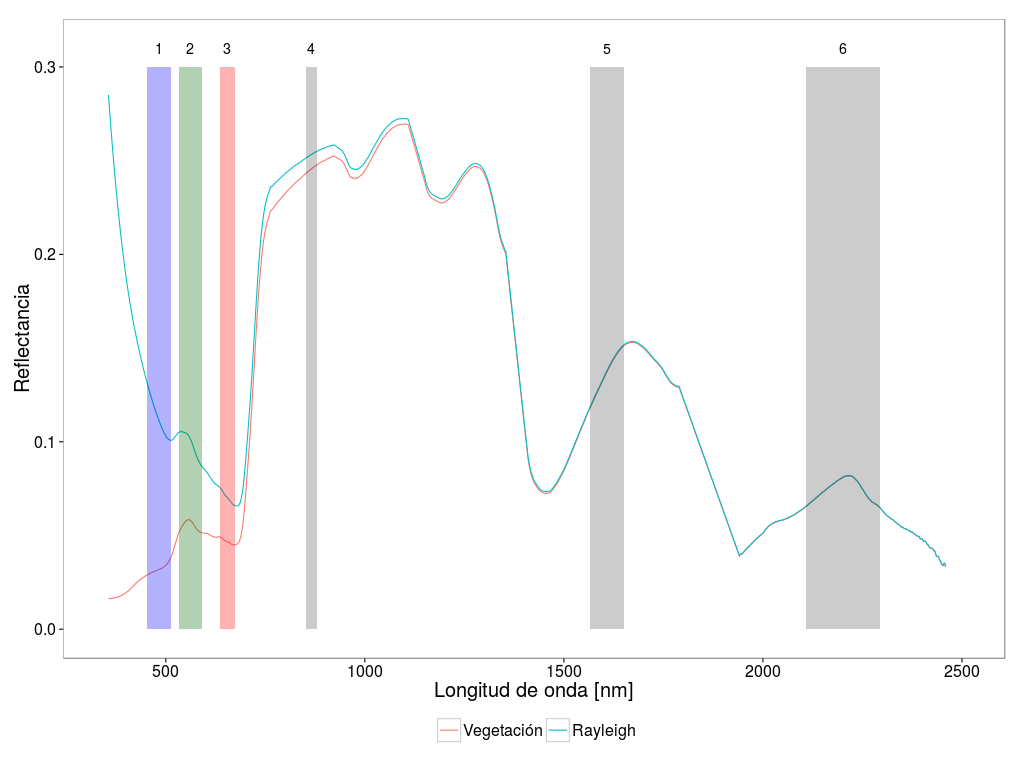
\includegraphics[width=0.8\textwidth]{imagenes/rayleigh.png}
  \caption{Variacion de la firma espectral por dispersión de Rayleigh. \footfullcite{clark2007usgs}}
  \end{figure}
\end{frame}
%--- Next Frame ---%


\subsection{Aerosoles}

\begin{frame}{Aerosoles}
  \begin{itemize}
    \item Su presencia en la atmósfera no va a ser constante.
    \item Es de las contribuciones mas complicadas de modelar.
    \item Incluso si se sabe que cantidad de aerosoles hay es importante también saber de que tipo.
  \end{itemize}
\end{frame}
%--- Next Frame ---%

\begin{frame}{Aerosoles}
  En un modelo de juguete
  \begin{equation}
    L = L_0 \left( \frac{\lambda}{\lambda_0} \right)^{-\alpha}
  \end{equation}
  donde $4 > \alpha > 1$ disminuye a medida que disminuye la visibilidad.
\end{frame}
%--- Next Frame ---%

\begin{frame}{Dispersión}
  \begin{exampleblock}{Porcentaje de dispersión típica}
    Para Landat 5 - TM
    \begin{figure}
      \begin{tabular}{l c c}
        Banda & Rayleigh  & Aerosol    \\
        $490\pm60 nm$& $\nearrow$ 0.064 - 0.080   & $\nearrow$ 0.007 - 0.048 \\
        $575\pm75 nm$& $\nearrow$ 0.032 - 0.040   & $\nearrow$ 0.006 - 0.040  \\
        $670\pm70 nm$& $\nearrow$ 0.018 - 0.020   & $\nearrow$ 0.005 - 0.034 \\
        $837\pm107 nm$& $\nearrow$ 0.007 - 0.009  & $\nearrow$ 0.003 - 0.023 \\
        $1692\pm178 nm$& $\nearrow$ 0.000 - 0.001  & $\nearrow$ 0.001 - 0.007 \\
        $2190\pm215 nm$& -                         & $\nearrow$ 0.001 - 0.004 \\
      \end{tabular}
    \end{figure}
  \end{exampleblock}
\end{frame}
%--- Next Frame ---%

\subsection{Absorciones}

\begin{frame}{Composición de la atmósfera}
  \begin{figure}
  \centering
  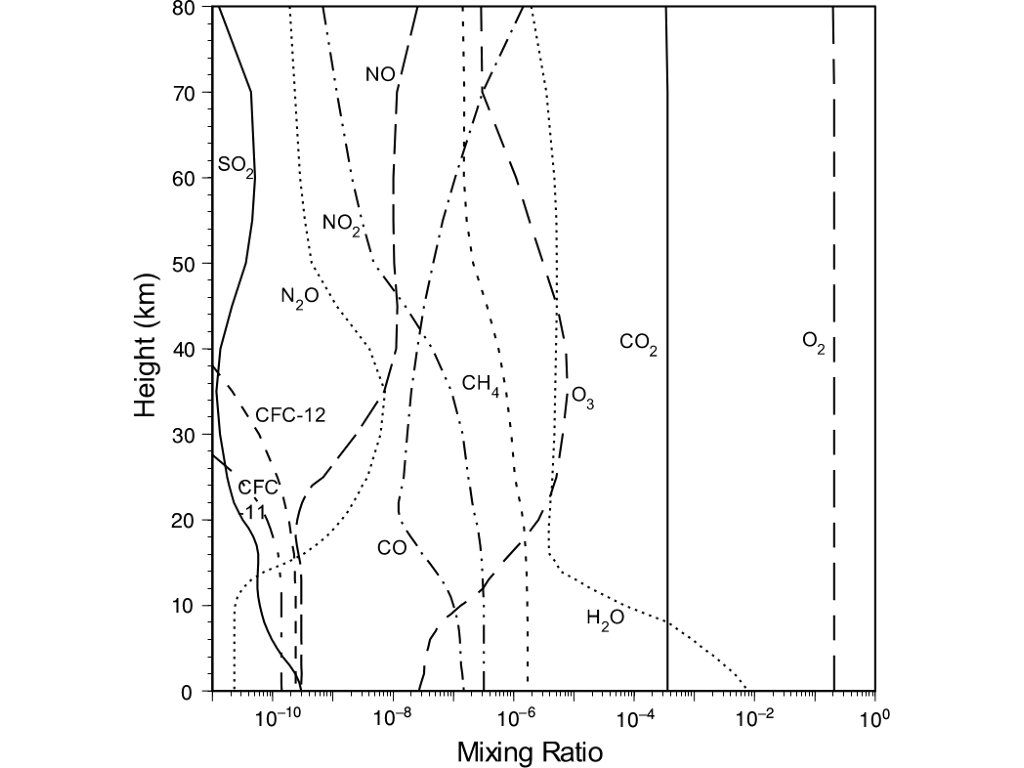
\includegraphics[width=0.8\textwidth]{imagenes/composicion.png}
  \caption{Composición de la atmósfera.\footfullcite{liou2002introduction}}
  \end{figure}
\end{frame}
%--- Next Frame ---%

\begin{frame}{Ventanas atmósfericas}
  \begin{figure}
  \centering
  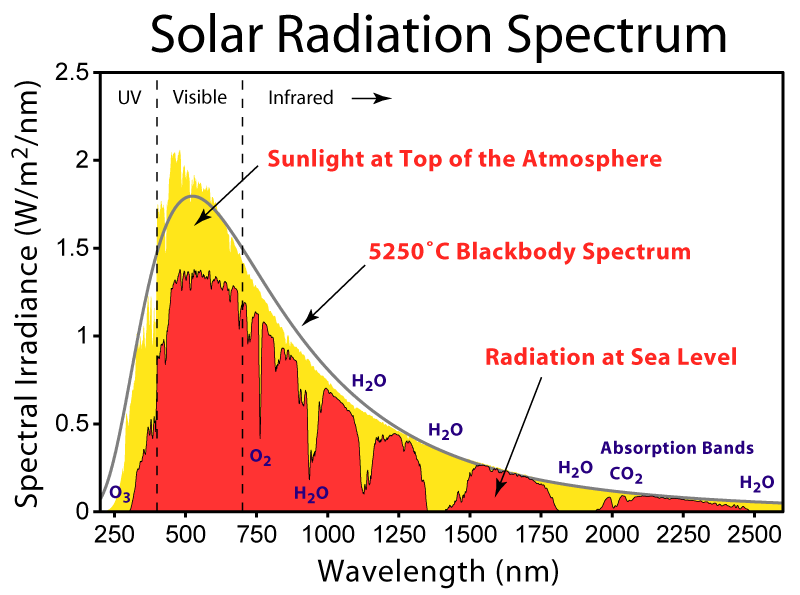
\includegraphics[width=0.7\textwidth]{imagenes/solar_spectrum.png}
    \caption{Comparación entre la irradiancia solar a tope de la atmósfera y de la cobertura.\footfullcite{solar_spectrum}}
  \end{figure}
\end{frame}
%--- Next Frame ---%

\begin{frame}{Absorciones}
  \begin{figure}
  \centering
  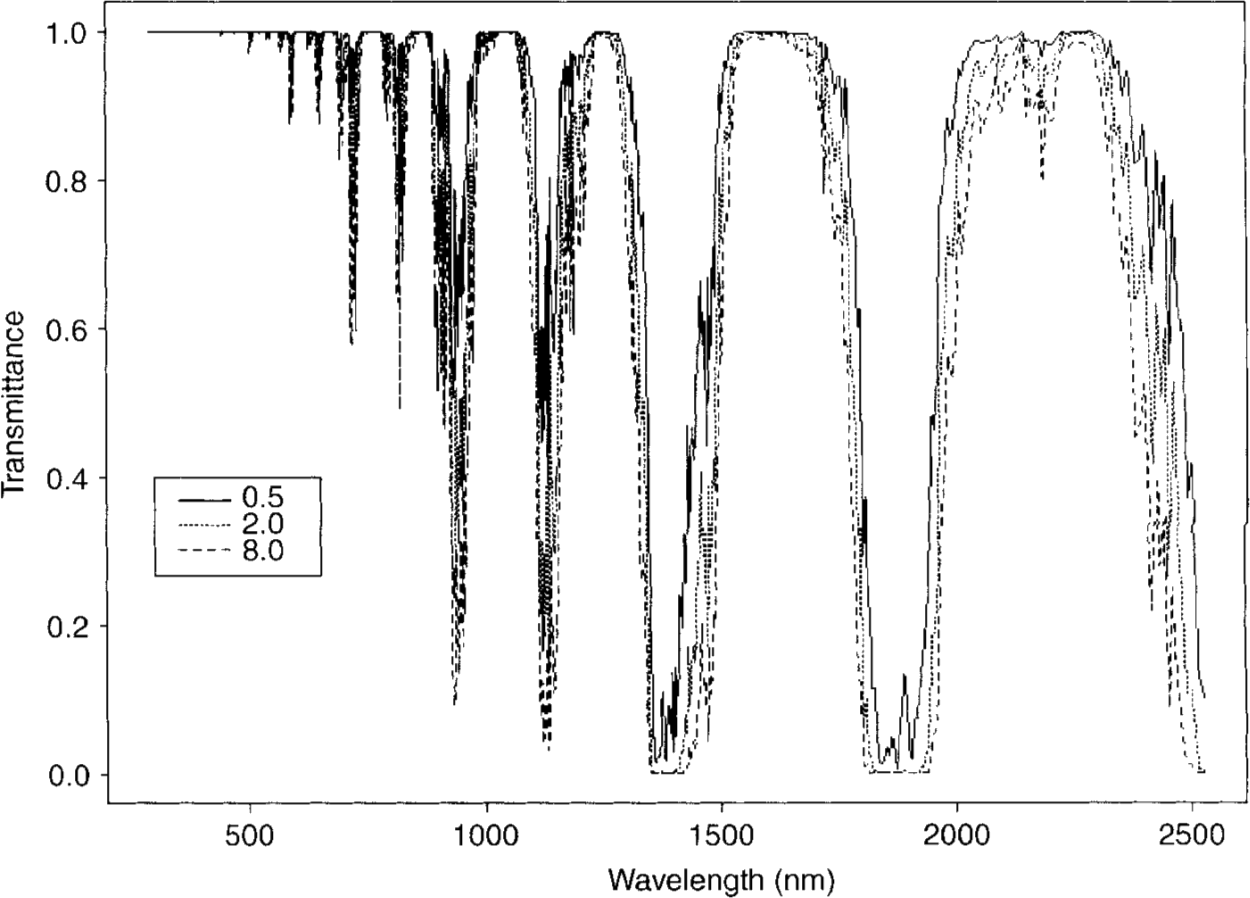
\includegraphics[width=0.8\textwidth]{imagenes/vapor.png}
  \caption{Variaciones de la absorción por contenido de vapor de agua.\footfullcite{liang2005quantitative}}
  \end{figure}
\end{frame}
%--- Next Frame ---%


\begin{frame}{Absorciones}
  \begin{exampleblock}{Porcentaje de absorción típica}
    Para Landat 5 - TM
    \begin{figure}
      \begin{tabular}{l c c}
        Banda & Ozono  & Vapor de agua    \\
        $490\pm60 nm$& $\searrow$ 1.5\% - 2.9\%     & -  \\
        $575\pm75 nm$& $\searrow$ 5.2\% - 13.4\%    & $\searrow$ 0.5\%-3\%  \\
        $670\pm70 nm$& $\searrow$ 3.1\% - 7.9\%     & $\searrow$ 0.5\%-3\%  \\
        $837\pm107 nm$& -                 & $\searrow$ 3.5\%-14\%  \\
        $1692\pm178 nm$& -                 & $\searrow$ 5\%-16\% \\
        $2190\pm215 nm$& -                 & $\searrow$ 2.5\%-13\% \\
      \end{tabular}
      \caption{Variaciones de absorvancia por contenidod de ozono y vapor de agua. \footfullcite{vermote49atmospheric}}
    \end{figure}
  \end{exampleblock}
\end{frame}
%--- Next Frame ---%

\begin{frame}{Absorciones}
  \begin{figure}
  \centering
  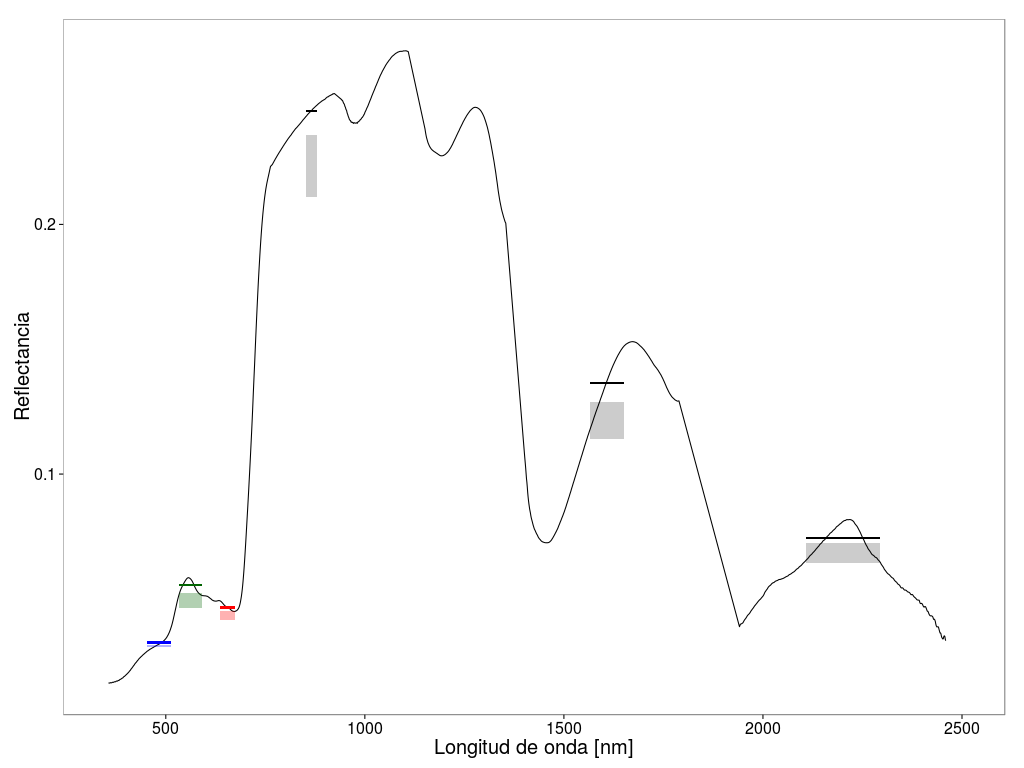
\includegraphics[width=0.7\textwidth]{imagenes/abs_veg_esp.png}
  \caption{Comparación entre la firma espectral y la respuesta espectral para vegetación con errores por absorciÓn de ozono y vapor de agua.\footfullcite{clark2007usgs}}
  \end{figure}
\end{frame}
%--- Next Frame ---%

\section{Métodos de resolución}
\begin{frame}{Reflectancia}
  \begin{equation}
    \rho_{TOA} = \frac{\pi L}{\cos \theta_z E_0}
  \end{equation}
\end{frame}
%--- Next Frame ---%

\subsection{Dark Object Substraction}
\begin{frame}{DOS}
  Esté método se apoya en suposiciones sobre las imágenes para estimar el valor de $L_P$.
\end{frame}
%--- Next Frame ---%

\begin{frame}{DOS}
  \begin{figure}
  \centering
  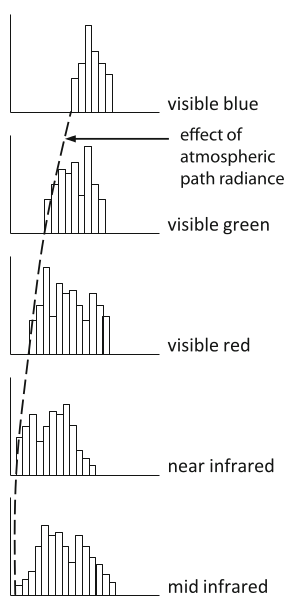
\includegraphics[width=0.30\textwidth]{imagenes/dos.png}
  \caption{Histogramas por banda mostrando el menor valor en cada una.\footfullcite{richards2013remote}}
  \end{figure}
\end{frame}
%--- Next Frame ---%

\begin{frame}{DOS}
  \begin{alertblock}{Importante}
    Estamos suponiendo que tenemos un cuerpo de reflectancia cero en cada banda dentro de la imagen.
  \end{alertblock}
\end{frame}
%--- Next Frame ---%

\begin{frame}{DOS}
  \begin{equation}
    \rho_{TOC} = \rho_{TOA} - \rho_{TOA,min}
  \end{equation}
\end{frame}
%--- Next Frame ---%

\subsection{6S}
\begin{frame}{6S}
  En este método vamos a introducir datos sobre las condiciones de la atmósfera para calcular todos los parámetros para la corrección.
\end{frame}
%--- Next Frame ---%

\begin{frame}{6S}
  Vamos a necesitar
  \begin{itemize}
    \item La visibilidad meteorológica.
    \item Tipo de sensor.
    \item Ángulos cenital y azimutal.
    \item Fecha, hora, latitud y longitud.
  \end{itemize}
\end{frame}
%--- Next Frame ---%

\begin{frame}{6S}
  \begin{block}{Simulador}
    \texttt{http://6s.ltdri.org/pages/run6SV.html}
  \end{block}
\end{frame}
%--- Next Frame ---%

\begin{frame}{DOS}
  \begin{alertblock}{Importante}
    Poner mal los parámetros acá puede que de cualquier cosa.
  \end{alertblock}
\end{frame}
%--- Next Frame ---%

\begin{frame}{DOS}
  \begin{equation}
    \rho_{TOC} = \frac{A\rho_{TOA} + B }{1 + \gamma (A\rho_{TOA}+B)}
  \end{equation}\pause
  \begin{itemize}
    \item $A = 1/\alpha\beta$.
    \item $B = -\rho_I/\beta$.
    \item $\alpha$ Global gas transmitance.
    \item $\beta$ Total scattering transmitance.
    \item $\gamma$ Spherical albedo.
  \end{itemize}
\end{frame}
%--- Next Frame ---%
\section{Práctica}

\begin{frame}{Práctica}
  \begin{exampleblock}{Actividades prácticas de la primera clase}
    \begin{enumerate}
      \item Calibrar la imagen L1 a reflectancia a tope de la atmósfera.
      \item Corregir la imagen por el método DOS
      \item Corregir la imagen por el método del 6S.
      \item Comparar las firmas espéctrales.
    \end{enumerate}
  \end{exampleblock}
\end{frame}
%--- Next Frame ---%

\end{document}
